
After movement data were collected, we ran our analysis to compute volume rates for each exercise and form measurement for three selected exercises: jumping jacks, high marches, and squat jumps. Below we describe the data analysis procedures we performed. (The first step, omitted from the descriptions below, was essential data cleansing by deleting rows containing NULL values. The number of such rows did not exceed two per any of the data files, amounting to less than 0.002\% of the data.)

\subsubsection{Rate Calculations}
\textbf{Jumping Jacks}  \\
Jumping jacks consist of starting position (standing still, feet together) and jumping position (feet spread wide). To compute repetitions, we took the x coordinates of a participant's left and right feet and plotted the absolute difference between the two coordinates over time, as shown in figure below.
%%%%%%%%%%%%%%%%%%%%%%%%%%
\begin{figure} [htp]
	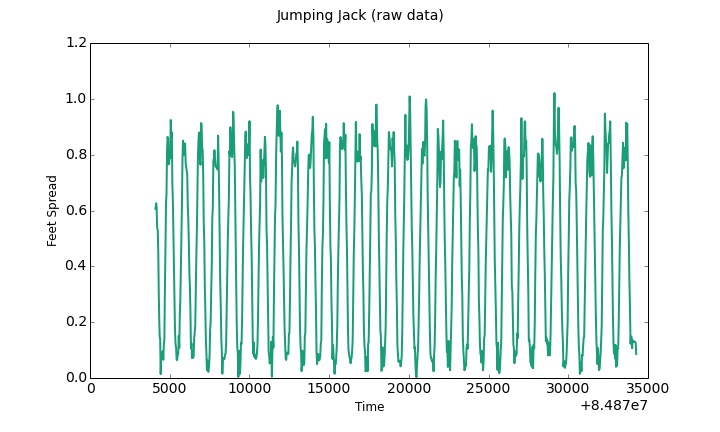
\includegraphics[width=0.5\textwidth]{images/jj_raw}
%\caption{Arm Circles Results}
\end{figure}
%%%%%%%%%%%%%%%%%%%%%%%%%%
Each of the lows corresponds to a starting position and each of the peaks corresponds to a jumping position. Therefore, to count the number of repetitions, it suffices to count the number of peaks. Given the relative noisiness of the original data set, a naive algorithm to compute local maxima would yield an excessive number of false positives, necessitating further data processing. We experimented with two methods: smoothing and robust peak detection. In terms of smoothing, we applied a third-order spline interpolation. For robust peak detection, we classified a point as a local maximum if and only if it was preceded by a value lower than some delta, using an algorithm provided by Eli Billauer \cite{Billauer}. The best value of delta was determined by trial-and-error using our training data set consisting of three subjects (this data set was kept separate from our study data set). While each of theses methods led to significant improvements by itself, as determined by a dramatic reduction in the number of false positives, we found that we obtained the best results when we used both techniques: First, we smoothed-out the data, and then we applied the peak detection algorithm. Figure below shows the curve after smoothing. To compute the rate, we took the number of detected peaks and divided by the duration of the exercise.
%%%%%%%%%%%%%%%%%%%%%%%%%%
\begin{figure} [htp]
	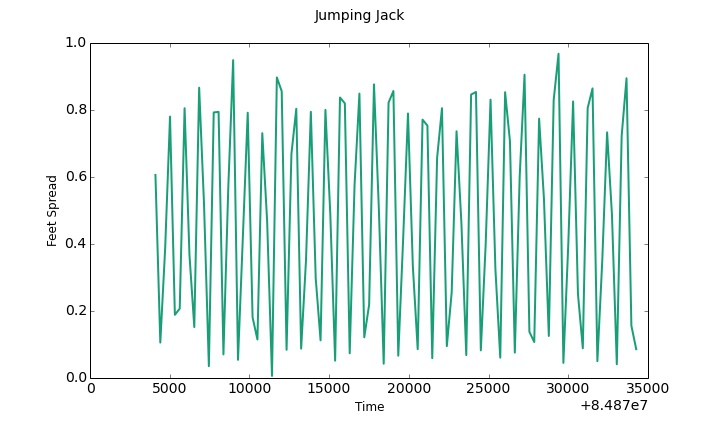
\includegraphics[width=0.5\textwidth]{images/jj}
%\caption{Arm Circles Results}
\end{figure}
%%%%%%%%%%%%%%%%%%%%%%%%%%

\textbf{Squat Jumps}  \\
Similarly to jumping jacks, squat jumps consist of two basic positions: regular squat (starting posture) and a jump. To measure repetitions, we took the average y-coordinate values of a participant's feet and plotted the averages over time. As anticipated, the data revealed a pattern with distinct peaks, corresponding to each of the jumps. Figure below shows the curve after smoothing.
%%%%%%%%%%%%%%%%%%%%%%%%%%
\begin{figure} [htp]
	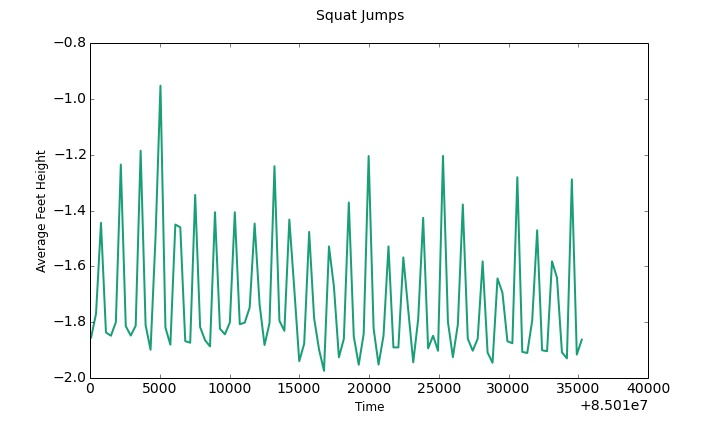
\includegraphics[width=0.5\textwidth]{images/sj}
%\caption{Arm Circles Results}
\end{figure}
%%%%%%%%%%%%%%%%%%%%%%%%%%
As in processing jumping jacks, we applied the peak detection algorithm on the smoothed-out curve, obtaining the number of repetitions, and then divided the count by exercise duration, to obtain the rate.

\textbf{High Marches} \\
High marches consist of alternatively kicking up as high as possible right and left feet, preferably while keeping knees straight. In analyzing high marches, we considered each leg separately. We took the y-coordinates of left and right ankles, smoothed-out the data and plotted it over time time. Figures below shows the curve for right ankle after smoothing. As in our earlier analyses, the number of peaks gave the number of repetitions, which we divided by duration to obtain the rate.
%%%%%%%%%%%%%%%%%%%%%%%%%%
\begin{figure} [htp]
	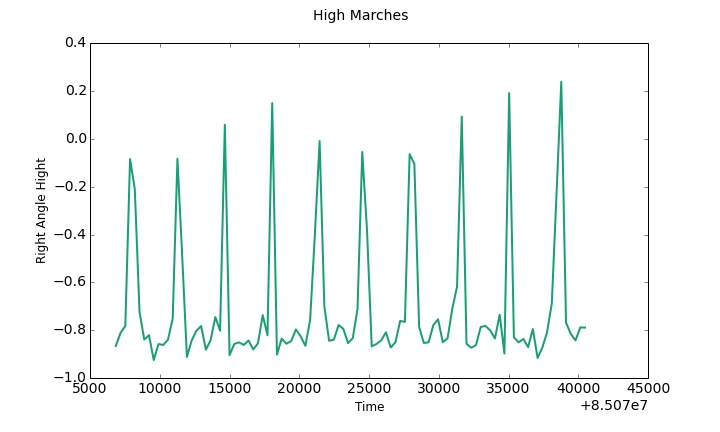
\includegraphics[width=0.5\textwidth]{images/hm}
%\caption{Arm Circles Results}
\end{figure}
%%%%%%%%%%%%%%%%%%%%%%%%%%

\textbf{Side-to-Side Jumps} \\
As the name suggests, side-to-side jumps consist of jumping from left to right, while keeping feet together. To calculate the rate, we took the average x-position of a participant's feet, smoothed-out the data, and plotted it over time. Then, we computed the number of peaks (corresponding to the time when the participant's feet were at rightmost point) and lows (corresponding to the time when the participant's feet were at the leftmost point). Figures below shows the curve after smoothing. We then used the sum of those numbers divided by exercise duration to obtain the rate.
%%%%%%%%%%%%%%%%%%%%%%%%%%
\begin{figure} [htp]
	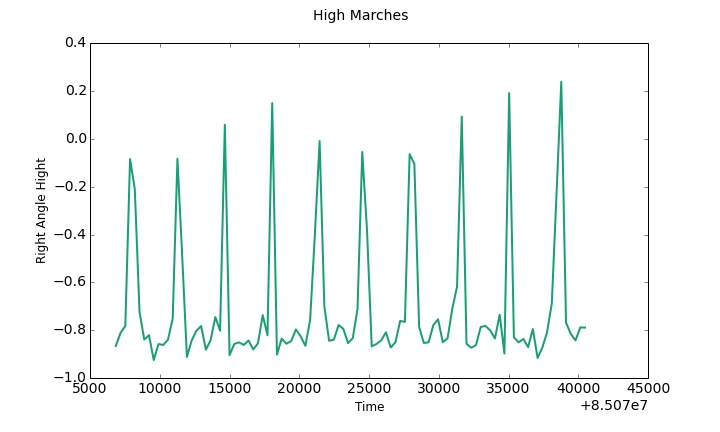
\includegraphics[width=0.5\textwidth]{images/hm}
%\caption{Arm Circles Results}
\end{figure}
%%%%%%%%%%%%%%%%%%%%%%%%%%

\textbf{Knee to Elbow} \\
To perform knee-to-elbow, a participant twists his torso while lifting his left knee to touch his right elbow, and then repeats on the opposite side, bringing up his right knee to touch his left elbow. From the standpoint of rate calculation, this exercise was more challenging to compute than any of the prior four. We took the x and y coordinates of a participant's left knee and right elbow. Then, we computed the Euclidean distance of these points over time. We repeated the same for right knee and left elbow and plotted the differences over time. Figures below shows the curve after smoothing. The lows correspond to the points when the participant's knee was closest to the corresponding elbow---indicating a completed repetition. Accordingly, we counted the number of lows on the smoothed-out curves for both knee-elbow pairs using the same strategy we used to detect peaks. A sum of those lows was then used to compute the rate.
%%%%%%%%%%%%%%%%%%%%%%%%%%
\begin{figure} [htp]
	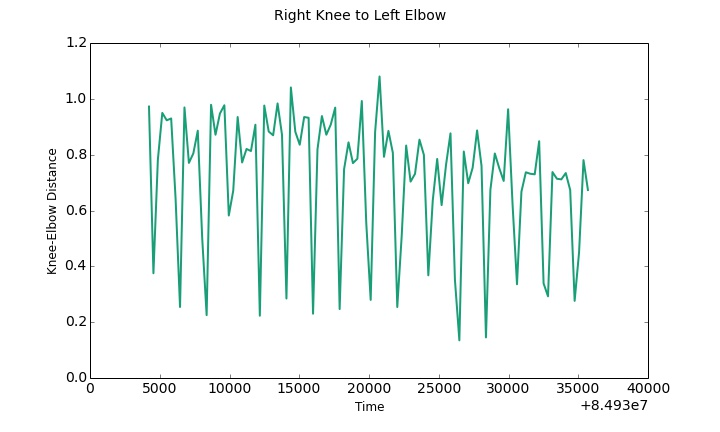
\includegraphics[width=0.5\textwidth]{images/ke}
%\caption{Arm Circles Results}
\end{figure}
%%%%%%%%%%%%%%%%%%%%%%%%%%

\textbf{Tuck Jumps} \\
Tuck jumps require the participant to jump as high as he or she can, raising his or her knees up. Here, we plotted the average y-position of the participant's knees over time; accordingly, each peak corresponds to a completed jump. Figures below shows the curve after smoothing. Similarly to the above-described procedures, we used the number of peaks to compute the rate.
%%%%%%%%%%%%%%%%%%%%%%%%%%
\begin{figure} [htp]
	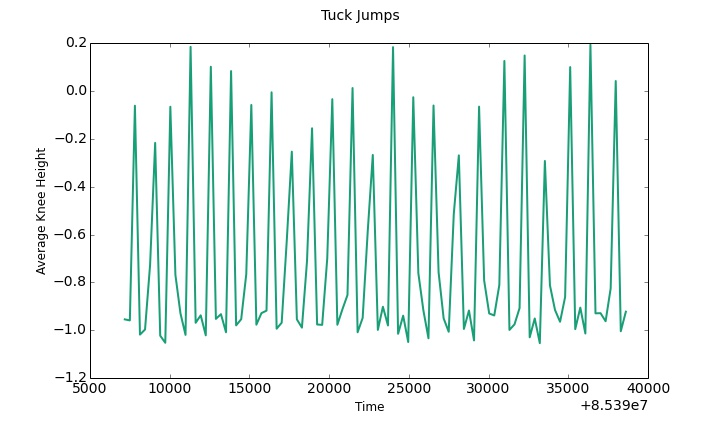
\includegraphics[width=0.5\textwidth]{images/tj}
%\caption{Arm Circles Results}
\end{figure}
%%%%%%%%%%%%%%%%%%%%%%%%%%

\textbf{Arm Circles} \\
In arm-circles starting position, the participant stands upright with arms extended to his or her sides, parallel to the ground. To perform the exercise, the participant makes circles with his or her outstretched arms, keeping elbows locked. To determine the number of repetitions, we observed that participant’s hand follows a roughly circular trajectory in the yz-plane. During a single circular traversal, a hand reaches exactly one minimum and maximum y and z position. Therefore, we plotted the smoothed-out the z and y positions for each wrist and computed the count of peaks and lows for each, dividing by two to obtain number of repetitions per wrist. Figures shows the curve for right wrist after smoothing. (While it would have been computationally simpler to consider only one of the dimensions---y or z---for the purposes of counting, such estimation could be easily deceived by up-down or front-back movement instead of the proper circular one.) We then took the average of the per-wrist repetition counts to compute the overall rate for this exercise.
%%%%%%%%%%%%%%%%%%%%%%%%%%
\begin{figure} [htp]
	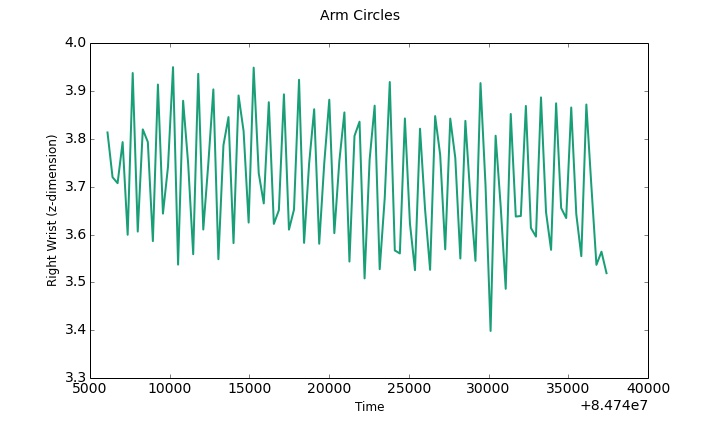
\includegraphics[width=0.5\textwidth]{images/ac}
%\caption{Arm Circles Results}
\end{figure}
%%%%%%%%%%%%%%%%%%%%%%%%%%

\subsubsection{Form Measurement}

In addition to counts, we developed ways to compute form metrics for select three exercises---jumping jacks, high marches, and squat jumps. We describe our methodology below.

\textbf{Jumping Jacks} \\
A proper form for jumping jacks demands straight knees throughout the exercise, wide leg spread in the jumping position, and complete retreat to the starting position where feet are touching. We noticed that all of these characteristics closely correlate with the magnitude of the difference between a participant's right and left feet x positions. For instance, a participant cannot achieve as large a spread in the jumping position if his knees are not straight compared to when his knees are locked. In addition, the differences will be smaller if the participant fails to retreat completely to the starting position before performing another jump. Accordingly, we used the average difference of the x coordinates of a participant's left and right feet, normalized by the his height, to gauge relative form between participants.

\textbf{High Marches} \\
To perform high marches properly, a participant needs to kick up as high as possible while keeping her knees straight. Unfortunately, the knee data have shown to be too noisy to make fine deductions such as the relative straightness of knees. However, we observed that bent knees necessarily lead to lower feet y-position during kick-ups compared to when the knees are straight. Therefore, we used the average foot height per each rep, normalized by the participant's height, to compute the relative form metric for high marches.

\textbf{Squat Jumps} \\
Squat jumps demand that the participant jumps as high as possible while bringing his or her knees as close to his or her chest as possible. Accordingly, to compute a metric that could be used to compare squat jump form across multiple participants, we took the average in-jump knee height for each participant, normalized by height.

